% !TEX root = main.tex
\documentclass[twocolumn]{article}
\usepackage[a4paper,margin=1in]{geometry} 
\usepackage{lmodern}
\usepackage{setspace}
\usepackage{mathptmx}
\usepackage{algorithm}
\usepackage{algpseudocode}
\usepackage{amsmath}
\usepackage{booktabs}
\usepackage{arydshln}
\usepackage{float}
\usepackage{cite}
\usepackage{multirow}
\usepackage{graphicx}
\usepackage{url}
\usepackage{import}
\usepackage{xcolor}

% \setcounter{secnumdepth}{0}

\title{\vspace{-1.5cm}\huge Words That Matter:\\ Vocabulary Pruning in ModernBERT}
\author{
Wout De Rijck\\[0.5em]
\small{Supervisors:} \normalsize Prof. Dr. Ir. Thomas Demeester, \normalsize Prof. Dr. Ir. Chris Develder\\
\small{Councellor:} \normalsize Dr. Ir. Karel D'Oosterlinck
}
\date{} % No date

\begin{document}
\maketitle


\textbf{Abstract:} Large language models (LLMs) require substantial computational and memory resources, limiting their utility in resource-constrained environments. 
ModernBERT is a smaller encoder-only language model that excels at various tasks while being computationally highly efficient. 
In this work, we study how much more ModernBERT can be compressed while retaining accuracy on any given task.
Specifically, we introduce a series of very simple vocabulary pruning techniques that target the embedding layer. We compare the resulting accuracy with LoSparse, a state-of-the-art gradient-based pruning technique that targets the encoder layers.
For parameter reductions up to $\sim$20\%, our much simpler vocabulary pruning technique outperforms LoSparse, retaining up to 97.6\% of ModernBERT's performance across various tasks, compared to LoSparse's 96.2\%.
The strong performance of our simple technique indicates that task-specific pruning can meaningfully increase the efficiency of ModernBERT, an already highly efficient model. Additionally, our results suggest that state-of-the-art encoder-layer pruning can fall short of simple embedding-layer pruning.
We provide open-source implementations of all pruning methods and evaluation tools to support further research in this area. (\url{https://github.com/WoutDeRijck/vocab-pruning.git})

\textbf{Keywords:} vocabulary pruning, ModernBERT, encoder-only model, model compression, embedding-layer, task-specific pruning, TF-IDF

\section{Introduction}
Language models need to be efficient for optimal deployment.
Efficiency can be assessed in several dimensions, including inference latency, throughput, energy consumption, parameter count, and memory usage\cite{yuan2025efficientllm}.
In this work, we study how to optimally reduce the memory footprint of language models by removing unimportant vocabulary tokens from the embedding layer, resulting in faster model loading, reduced deployment costs, and improved accessibility for edge devices or resource-constrained environments.

\begin{figure}[t]
\centering
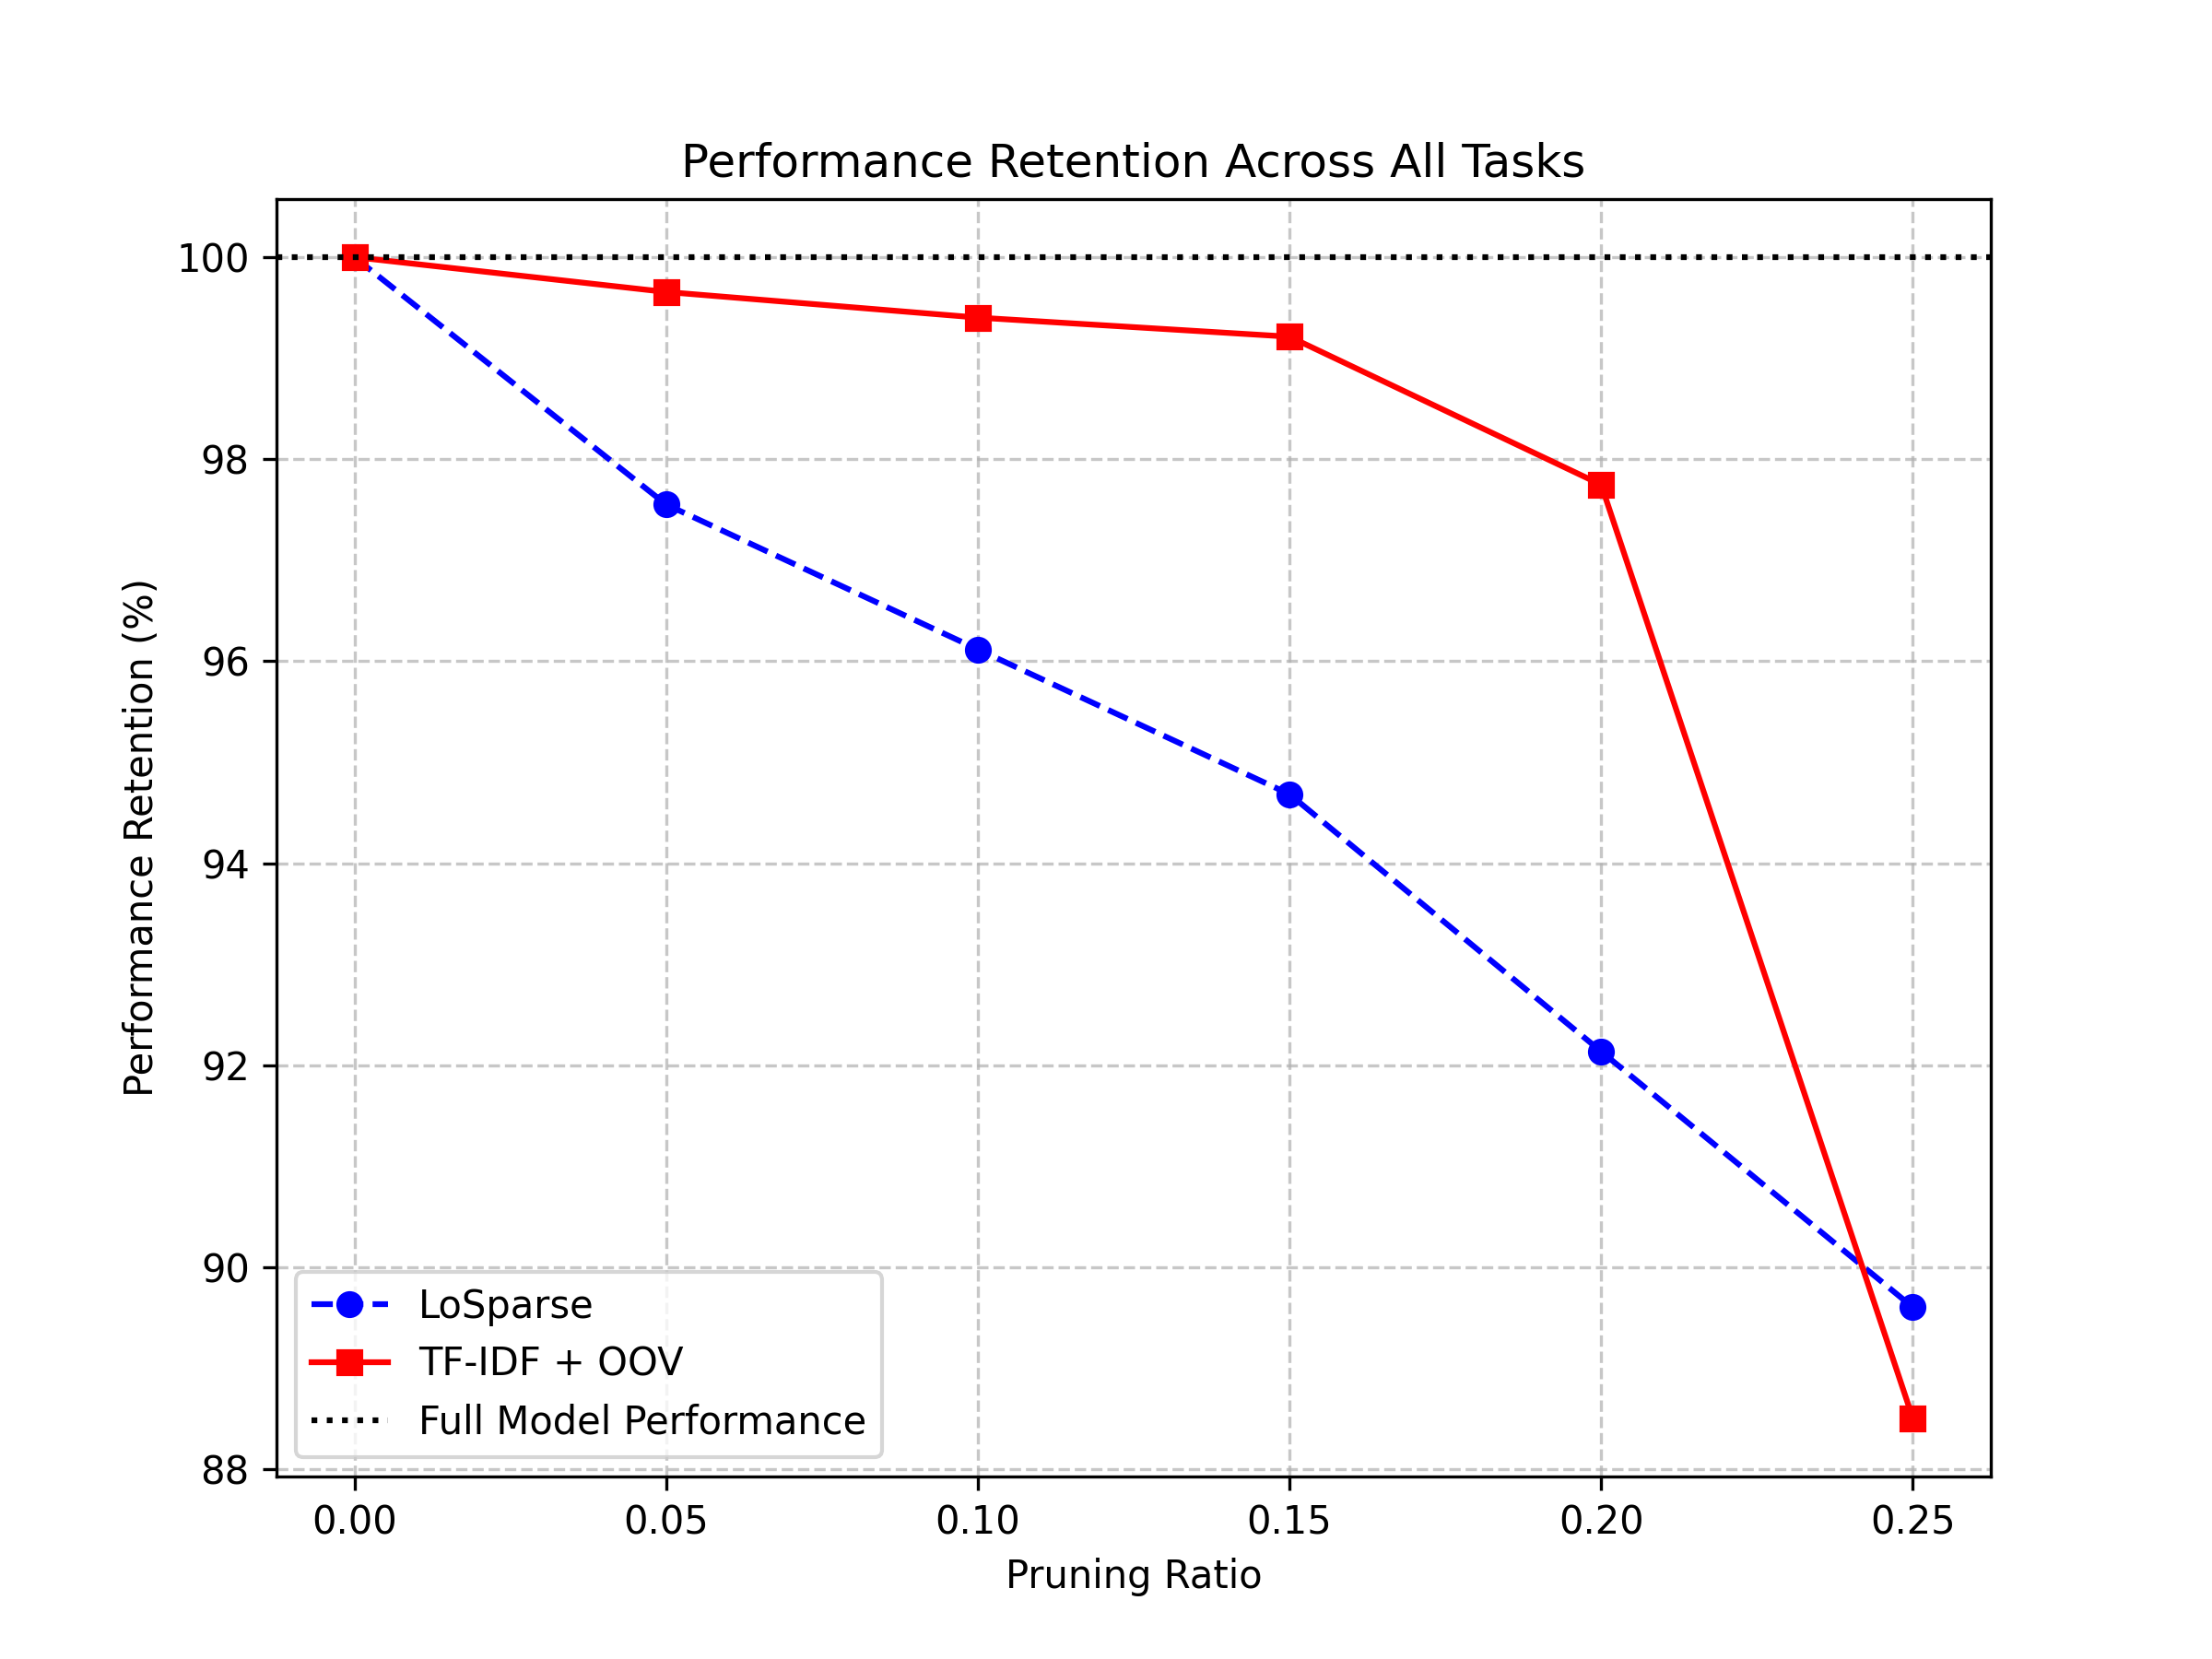
\includegraphics[width=\columnwidth]{images/performance_retention.png}
\caption{Simple vocabulary pruning techniques retain \raisebox{0.2ex}{\scalebox{0.8}{$>$}}97\% of ModernBERT's performance while removing $20\%$ of total parameters across eight GLUE benchmark tasks. Our vocabulary pruning removes tokens based on their importance using \textit{TF-IDF}, with Out-of-Vocabulary (OOV) handling that maps removed tokens to semantically similar retained ones, substantially outperforming LoSparse---a state-of-the-art gradient-based encoder pruning method. Pruning ratio represents the fraction of total parameters removed from the model, limited to $0.25$ since the embedding layer constitutes $25.95\%$ of all model parameters, representing the theoretical maximum for vocabulary-only pruning.}
\label{fig:pruning_retention}
\end{figure}

ModernBERT \cite{warner2024modernbert} stands out as one of the most lightweight and optimized encoder-only transformers available. It integrates several architectural and training innovations while maintaining robust downstream performance. Despite these advancements, we investigate whether ModernBERT's efficiency can be further enhanced through parameter pruning. Given ModernBERT's inherent efficiency, optimal pruning strategies could yield exceptionally efficient models.

Specifically, we explore task-specific weight pruning, as ModernBERT is intended to be finetuned on specific tasks for optimal behavior (unlike more general-purpose decoder-only models that can utilize in-context learning). We hypothesize that simple task-specific pruning of the embedding matrix can be highly efficient, as many tokens can be irrelevant for any specific downstream task, and the embedding layers counts for a significant portion ($\sim$25\%) of the total parameters \cite{yang2022taskspecific}.

We explore a series of simple vocabulary pruning heuristics on a range of Natural Language Processing tasks, including linguistic acceptability, sentiment analysis, paraphrase detection, semantic similarity, question answering, and natural language inference, as covered by the GLUE benchmark \cite{wang2018glue}. For any task, we first apply vocabulary pruning to the base ModernBERT model and subsequently finetune the pruned model. We compare these vocabulary pruning techniques with LoSparse \cite{li2023losparse}, a state-of-the-art gradient-based pruning technique that targets the encoder layers.


Our results show that TFIDF-based vocabulary pruning (with frequencies computed from the target task's training dataset) outperforms encoder-layer pruning (LoSparse) for compression ratios up to 20\%, maintaining 97.6\% of ModernBERT's original performance while removing 77.34\% of embedding parameters (see Figure \ref{fig:pruning_retention}). This shows that substantial efficiency gains can be achieved with virtually no performance loss using a simple, offline pruning technique. Beyond 20\% compression, performance drops sharply as we approach the embedding layer's parameter limit (25.95\% of total model parameters), 
% while LoSparse maintains more stable performance at higher ratios.
while LoSparse maintains more stable performance at higher ratios, since it can continue pruning across the larger encoder layers (74.05\% of total parameters). 
Unlike LoSparse, which requires computationally expensive gradient-based optimization, our vocabulary pruning operates as a pre-finetuning step with minimal overhead.


Our results indicate that the memory footprint of light-weight models, such as ModernBERT, can still be significantly improved.  We open-source all our code.

\section{Related work}
Model compression techniques enhance the efficiency of large language models (LLMs) by reducing their size and computational requirements.
% 
These techniques can be broadly categorized into four primary methods~\cite{wan2023efficient, park2024comprehensive, cheng2017survey, mishra2020survey, xailient2021compression}:
(i) \textbf{quantization}, which reduces the numerical precision of model weights \cite{gholami2021survey};
(ii) \textbf{parameter pruning}, which eliminates redundant or less important connections and neurons to create sparser models with fewer parameters \cite{cheng2023survey};
(iii) \textbf{low-rank approximation}, which decomposes weight matrices into lower-dimensional representations that capture essential information while requiring fewer parameters~\cite{Hu2021LoRA}; and
(iv) \textbf{knowledge distillation} transfers knowledge from larger teacher models to smaller student models, enabling competitive performance with reduced architecture size ~\cite{Hinton2015Distillation}.


%can you give an example here?
%Misschien niet nodig voor de paper maar heel goed om je expertise te tonen in de full thesis
The model compression techniques described above are complementary and can be combined to achieve optimal compression \cite{muralidharan2024compact, han2015deep, choukroun2019low}.
This work focuses on parameter pruning techniques to reduce model size while preserving performance. The rest of this section gives an overview of the most important parameter pruning techniques.


% In de thesis kan je veel content "winnen" door LoSparse volledig uit te leggen, kan dan ook beknopt in de paper komen.
% Maar vooral belangrijk voor de thesis om de equations uit te schrijven als je content nodig hebt
\textbf{Encoder-Layer Pruning methods} remove less critical parameters within the encoder to reduce model size while maintaining acceptable accuracy. A representative state-of-the-art method is LoSparse~\cite{li2023losparse}, which decomposes each weight matrix into a low-rank component and a sparse residual. During finetuning, LoSparse calculates the importance of each weight by multiplying it by its gradient, which is resource-intensive.

Attention-head pruning~\cite{michel2019sixteen} removes entire attention heads, whereas LoSparse removes entire neurons (i.e., rows in weight matrices). Movement pruning~\cite{sanh2020movement} applies gradient-guided masking to gradually zero out low-importance weights during finetuning. LayerDrop~\cite{fan2020layerdrop} introduces structured dropout, allowing entire transformer layers to be stochastically removed during training and optionally pruned at inference.

These encoder-layer pruning methods differ in their granularity and strategy—targeting individual weights, attention heads, or full layers. LoSparse stands out as a strong baseline for encoder-level pruning~\cite{pmlr-v235-li24bi, huang2023awesome, ren2025llmcompression}.


% \paragraph{Embedding-Layer Pruning methods}
\textbf{Embedding-Layer Pruning methods} reduce the memory footprint of the embedding layer, which can comprise up to 20-30\% of a model's parameters. These methods can be categorized into two main strategies: embedding compression and vocabulary pruning.

\textit{\textbf{Embedding compression}} reduces the dimensional representation of the embeddings. LightToken~\cite{wang2023lighttoken} is a model- and task-agnostic framework for compressing the token embedding layers. It uses a combination of low-rank approximation, a residual binary autoencoder, and a novel compression loss to drastically reduce embedding size. 

\textit{\textbf{Vocabulary Pruning Techniques}} are a specialized form of embedding pruning that removes rarely used or task-irrelevant tokens.

The simplest approach is to drop unused tokens. TextPruner~\cite{shen2022textpruner} scans a corpus and removes tokenizer tokens not present in the target text. This can reduce BERT$_{\text{BASE}}$'s embedding matrix by up to 47\% without compromising performance.

For multilingual models, most of the parameters are located in the embedding layer, language-specific pruning has proven effective. Abdaoui et al.~\cite{abdaoui2020load} showed that trimming unused language tokens from mBERT can achieve a 45\% parameter reduction with comparable accuracy on XNLI. Similarly, BLADE~\cite{nair2023blade} builds pruned bilingual models containing only tokens from target languages, reducing parameters by $\sim$36.5\% versus full mBERT while speeding up training by $\sim$30\% and inference by $\sim$55\%.

% These findings consistently demonstrate that vocabulary pruning is an effective way to tailor models to specific domains or languages with minimal performance impact.
While simply removing embeddings for unseen (i.e., never‑used) tokens has proven to be effective, we show one can go substantially further by additionally ranking and pruning low‑utility tokens. 

To our knowledge, this is the first study to (i) rigorously evaluate a range of importance heuristics in a single framework, (ii) incorporate OOV‑aware mapping to preserve semantic fidelity of pruned tokens, and (iii) apply vocabulary pruning atop ModernBERT thereby demonstrating the practical benefits of embedding‑layer reduction in resource‑constrained settings.

\newpage
% \section{Method}
% \section{Token-level encoder compression}
\section{\fontsize{13}{15.6}\selectfont Task-Specific Vocabulary Pruning}
Our vocabulary pruning method is straightforward: we first remove all tokens that do not appear in our training dataset, then we eliminate an additional percentage of the remaining tokens based on importance scores. 
Optionally, we cluster removed tokens into groups and add the cluster centroids back into the vocabulary to handle out-of-vocabulary (OOV) cases during inference.

We apply this method to ModernBERT, where the embedding layer accounts for approximately 25\% of the model's parameters. This approach is based on the observation that tokens in a vocabulary have varying importance for downstream tasks, and that certain tokens can be selectively removed with minimal impact on performance. 

In contrast to methods that require resource-intensive post-pruning finetuning, the proposed vocabulary pruning approach operates as a \textbf{pre-finetuning offline pruning} step in the model adaptation pipeline.
It requires only the training dataset to determine token importance and prune the vocabulary, without needing gradients from finetuning, allowing the resulting pruned model to be finetuned with minimal computational overhead.


We compute token importance scores using either attention-based (Algorithm \ref{alg:pre_ft_pruning}, lines 2-4) or statistical approaches (line 6) via \texttt{compute\_importance\_scores}, then sort and select the top $k$ tokens based on the pruning ratio $p$ (lines 7-9).
The least important tokens are pruned from the embedding layer, and the embedding matrix is reconstructed using only the retained tokens (\texttt{rebuild\_model\_with\_vocab}, line 13), yielding a smaller model. 
To recover the loss of throwing away tokens, semantic clustering can be applied with \texttt{cluster\_pruned\_tokens} to map pruned tokens to semantically similar retained tokens (lines 10-12). 
This approach front-loads the pruning work to the pre-finetuning phase, meaning the actual finetuning process remains unchanged and operates on an already-reduced model. With a pruning ratio of 0, our algorithm defaults to standard finetuning of the base model.

\begin{algorithm}[H]
\footnotesize
\caption{Pre-Finetuning Vocabulary Pruning}
\label{alg:pre_ft_pruning}
\begin{algorithmic}[1]
\Require Model $M$ with vocab $V$, dataset $D$, pruning ratio $p$
\Ensure Pruned model $M'$ with reduced vocabulary
\State $V_s \gets \text{get\_special\_tokens}(M)$ \Comment{[CLS], [SEP]}
\If{using attention scoring}
    \State $M_\text{ft} \gets \text{finetune}(M, D)$ \Comment{Finetune model on task}
    \State $s \gets \text{compute\_attention\_scores}(M_\text{ft}, D, V)$ 
\Else
    \State $s \gets \text{compute\_token\_scores}(D, V)$
\EndIf
\State $V_{\text{sorted}} \gets \text{sort}(V \setminus V_s, s, \text{desc})$
\State $k \gets \lfloor (1-p) \cdot |V_{\text{sorted}}| \rfloor$ \Comment{Number of tokens to keep}
\State $V_{\text{keep}} \gets V_s \cup V_{\text{sorted}}[1:k]$
\If{using OOV handling}
    \State $\text{clusters} \gets \text{cluster\_pruned\_tokens}(V \setminus V_{\text{keep}})$
    \State $\text{oov\_map} \gets \text{map\_pruned\_to\_representatives}(\text{clusters})$
\EndIf
\State $M' \gets \text{rebuild\_model\_with\_vocab}(M, V_{\text{keep}}, \text{oov\_map})$
\State \Return $M'$
\end{algorithmic}
\end{algorithm}



\begin{table*}[h]
\centering
\scriptsize
\setlength{\tabcolsep}{9pt}
\begin{tabular}{l@{\hspace{25pt}}ccccccccc}
\toprule
& \multicolumn{2}{c}{\textbf{Single Sentence}} & \multicolumn{3}{c}{\textbf{Paraphrase and Similarity}} & \multicolumn{3}{c}{\textbf{Natural Language Inference}} & \multirow{2}{*}{\makebox[-20pt][c]{\vrule width 0.5pt height 175pt}\hspace{35pt}} \\
\cmidrule(lr){2-3} \cmidrule(lr){4-6} \cmidrule(lr){7-9}
\textbf{Method} & \textbf{SST-2} & \textbf{CoLA} & \textbf{MRPC} & \textbf{STS-B} & \textbf{QQP} & \textbf{MNLI} & \textbf{QNLI} & \textbf{RTE} & \textbf{AVG} \\
\midrule
\multicolumn{10}{l}{\textbf{Baseline}} \\
ModernBERT (Full) & 0.951 & 0.632 & 0.89 & 0.917 & 0.917 & 0.881 & 0.939 & 0.643 & 0.846 \\
\midrule
\multicolumn{10}{l}{\textbf{Vocabulary Pruning}} \\
Train Tokens Only & 0.950 & 0.630 & 0.861 & 0.917 & 0.917 & 0.883 & 0.915 & 0.639 & 0.839 \\
\textit{Parameter Reduction} & \textit{18.85\%} & \textit{22.61\%} & \textit{18.56\%} & \textit{18.76\%} & \textit{4.79\%} & \textit{6.74\%} & \textit{6.42\%} & \textit{17.06\%} & \textit{14.22\%} \\
\\ [-6pt]
\hdashline
\\[-6pt]
Random Selection & 0.911 & 0.470 & 0.798 & 0.845 & 0.780 & 0.504 & 0.669 & 0.566 & 0.693 \\
Clustering-Based & 0.894 & 0.188 & 0.752 & 0.696 & 0.871 & 0.683 & 0.833 & 0.566 & 0.685 \\
Attention-Based & \textbf{0.947} & 0.589 & \textbf{0.864} & 0.885 & 0.763 & 0.683 & 0.791 & 0.578 & 0.763 \\
Simple Frequency-Based & 0.943 & 0.467 & 0.812 & 0.905 & 0.904 & 0.858 & 0.902 & 0.546 & 0.792 \\
TF-IDF Based & 0.933 & 0.520 & 0.807 & 0.901 & 0.898 & 0.860 & 0.909 & 0.610 & 0.805 \\
\\ [-6pt]
\hdashline
\\[-6pt]
Simple Frequency + OOV & 0.938 & 0.540 & 0.828 & \textbf{0.906} & \textbf{0.915} & 0.858 & 0.907 & 0.615 & 0.813 \\
TF-IDF + OOV & 0.934 & \textbf{0.615} & 0.834 & 0.903 & 0.912 & 0.858 & \textbf{0.910} & \textbf{0.635} & \textbf{0.825} \\
\textit{Parameter Reduction} & \textit{20.25\%} & \textit{23.27\%} & \textit{20.02\%} & \textit{20.18\%} & \textit{20.02\%} & \textit{20.02\%} & \textit{20.02\%} & \textit{20.02\%} & \textit{20.48\%} \\
\midrule
\multicolumn{10}{l}{\textbf{Encoder Layer Pruning}} \\
LoSparse & 0.935 & 0.525 & 0.856 & 0.887 & \textbf{0.915} & \textbf{0.871} & 0.906 & 0.614 & 0.814 \\
\textit{Parameter Reduction} & \textit{20.16\%} & \textit{20.16\%} & \textit{20.16\%} & \textit{20.16\%} & \textit{20.16\%} & \textit{20.16\%} & \textit{20.16\%} & \textit{20.16\%} & \textit{20.16\%} \\
\bottomrule
\end{tabular}
\caption{Performance on GLUE dev set. ModernBERT is fine-tuned separately for each task. Scores are accuracies except for CoLA (Matthew's correlation), and STS-B (Pearson correlation). Notation "+ OOV" indicates pruning with out-of-vocabulary clustering. At 20\% parameter reduction, TF-IDF + OOV maintains 97.6\% of the original performance and outperforms LoSparse (0.825 vs 0.810 average score). OOV handling improves results by 2.0 percentage points on average.}

\label{tab:results}
\end{table*}
\subsection{Token Importance Analysis}
A critical challenge in vocabulary pruning is determining which tokens to retain and which to remove.
We explore several token importance estimation techniques, ranging from simple statistical methods to semantic analysis.

\textbf{Random Selection}
prunes tokens randomly without consideration for importance, serving as a baseline approach. In this method, tokens are selected for removal using uniform random sampling from the vocabulary.

\textbf{Clustering-Based}
preserves semantic diversity across the vocabulary using DBSCAN~\cite{wang2019dbscan} clustering to group similar token embeddings and keeping one representative per cluster. This leverages the property that embeddings with high cosine similarity typically have similar meanings\cite{mikolov2013efficient}, ensuring maximal semantic coverage with reduced vocabulary size.

\textbf{Frequency-Based} ranks tokens by their frequency in the training dataset, pruning the least frequently used tokens first. This approach is grounded in the heuristic that infrequent tokens contribute less to model performance ~\cite {li2024enhancing}.

We explore two frequency-based ranking methods. 
\textit{Simple Frequency} counts raw token occurrences in the training data, favoring common tokens.
\textit{TF-IDF} (Term Frequency-Inverse Document Frequency) balances token occurrence with discriminative power across documents. This method prioritizes tokens that appear frequently in specific documents but are rare across the corpus, capturing task-specific terminology while filtering out ubiquitous tokens that carry less semantic value. 

\textbf{Attention-Based}
leverages the attention mechanism of transformer models to identify potentially important tokens. The underlying principle is that tokens receiving higher attention during inference might be those the model relies on more when making predictions, offering a model-based perspective on token importance\cite{guo2024attention, kim2022learned, goyal2020powerbert, chen2021earlybert}. While attention scores do not necessarily imply causal relevance, they provide a task-specific signal that differs from simple statistical measures. The approach first finetunes the base model on the target task to learn task-specific attention patterns, then processes the dataset through this model to capture attention matrices from all layers and heads. It aggregates the attention each token receives across all its occurrences, and finally normalizes scores by token frequency to avoid bias toward common tokens.


\subsection{Out-of-Vocabulary Token Handling}
Vocabulary pruning raises an important question: how should the model process tokens that were removed from its vocabulary? Handling these out-of-vocabulary (OOV) tokens can recover performance lost due to pruning.
One option is to map all pruned tokens to a single UNK token, discarding their semantic information.
Alternatively, semantic clustering can be used to maintain some of the original meaning of pruned tokens.

% The clustering-based Out-Of-Vocabulary (OOV) handling process extracts embeddings for all pruned tokens and applies K-means clustering to group semantically similar tokens together. From each cluster, the token closest to the centroid is selected as a representative. During inference, when an OOV token is encountered, it is mapped to its assigned representative.
The clustering-based Out-Of-Vocabulary (OOV) handling process extracts embeddings for all pruned tokens and applies K-means clustering to group semantically similar tokens together. From each cluster, the token closest to the centroid is selected as a representative. While alternative clustering methods (e.g., DBSCAN) and representative selection strategies (e.g., averaging embeddings) could be explored, we focus on this approach for its simplicity and effectiveness. During inference, when an OOV token is encountered, it is mapped to its assigned representative.
The number of clusters (k) offers a tunable parameter to balance compression rate against semantic precision. While this approach adds a few more tokens back into the vocabulary, the intuition is that it can recover most of the performance lost during pruning.


After evaluating the different token importance metrics, we apply clustering-based OOV handling to the best-performing approach to further improve the results.

\begin{figure*}[t]
    \centering
    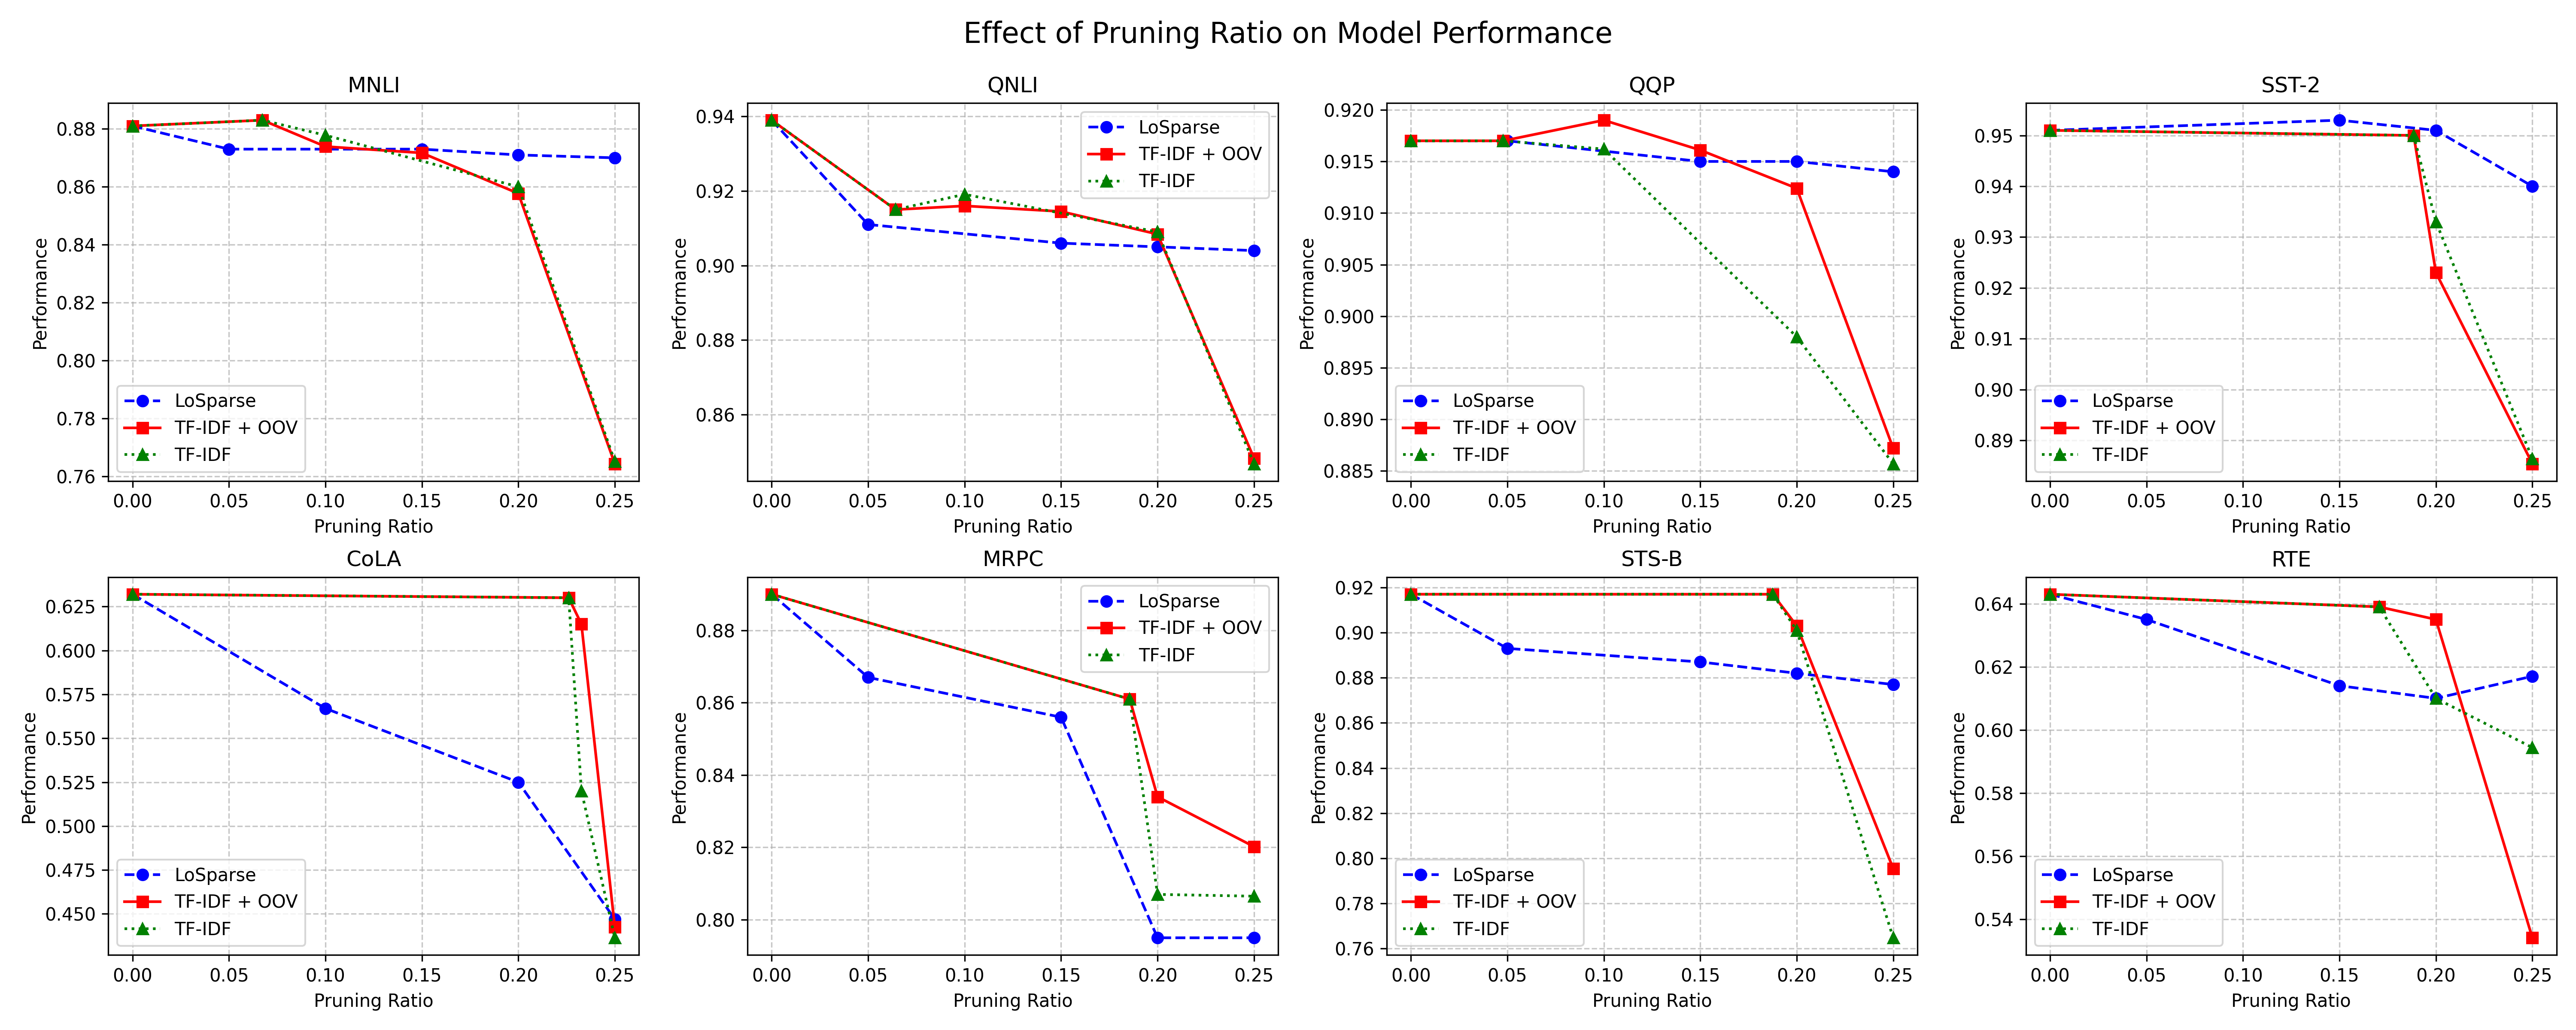
\includegraphics[width=\linewidth]{images/pruning_ratios.png}
    \caption{Performance comparison between vocabulary pruning (\textit{TF-IDF} with and without OOV) and encoder pruning (LoSparse). Vocabulary pruning outperforms LoSparse at lower pruning ratios (5-20\%), but performance drops sharply beyond 20\% as the embedding layer's parameter limit is reached, while LoSparse maintains more stable performance at higher compression rates.}
    \label{fig:pruning_ratio}
\end{figure*}

\section{Experiments}
We evaluate our vocabulary pruning methods across multiple natural language understanding tasks to assess their effectiveness. Additionally, we compare them to baseline approaches.

\textbf{For datasets and metrics,}
The General Language Understanding Evaluation (GLUE) benchmark\cite{wang2018glue} serves as our primary evaluation framework, comprising eight diverse NLP tasks: single-sentence tasks (SST-2\cite{socher2013recursive}, CoLA\cite{warstadt2019neural}), similarity/paraphrase tasks (MRPC\cite{dolan2005automatically}, STS-B\cite{cer2017semeval}, QQP\cite{qqp}), and inference tasks (MNLI\cite{williams2018broad}, QNLI\cite{rajpurkar2016squad}, RTE\cite{dagan2005pascal}). We report task-appropriate metrics: accuracy for most classification tasks, Matthew's correlation for CoLA, and Pearson correlation for STS-B. 


\textbf{As baselines,} 
we establish three baselines to evaluate our vocabulary pruning techniques: 
(i) \textit{ModernBERT (Full)} serves as the upper performance bound, using the complete 50,368-token vocabulary and all encoder parameters, finetuned on the training dataset of each task; 
(ii) \textit{LoSparse} provides an encoder-layer pruning baseline that uses low-rank and sparse factorization to preserve 80\% of parameters in encoder layers while maintaining the full embedding layer; 
(iii) \textit{Train Tokens Only} represents a simple vocabulary reduction approach that removes tokens not observed in finetuning data, achieving variable parameter reduction (4.79-22.61\%) depending on the dataset's vocabulary coverage.

\textbf{The results in}
Table \ref{tab:results} present a comprehensive evaluation across GLUE tasks for different pruning methods. 
% 
Vocabulary pruning achieves substantial parameter reduction (20.02-23.27\%) with minimal performance impact, with \textit{TF-IDF + OOV} maintaining 97.6\% of the original model's performance while reducing parameters by over 20\%. OOV handling mechanisms boost results compared to their non-OOV counterparts (+2.0 percentage points on average). 

The substantial performance degradation observed with random selection (0.693 average vs 0.846 baseline) demonstrates that strategic token selection is crucial for vocabulary pruning effectiveness.

Vocabulary pruning outperforms encoder-layer pruning (LoSparse) at lower pruning ratios (5-20\%), while only using simple statistics before finetuning, as shown in Figure \ref{fig:pruning_ratio}.
Specifically, a 20\% reduction in total parameters (77.34\% of vocabulary size) maintains competitive performance.


The efficacy of vocabulary pruning can be explained by the token-distribution: 20\% of tokens account for 80-94\% of all occurrences in training sets across GLUE tasks, as shown in Table \ref{tab:token_statistics}. This redundancy provides strong empirical justification for our approach. 

The table also highlights varying train-test vocabulary overlap across tasks, with unseen token percentages ranging from 0.14\% to 13.70\%. These high rates of unseen tokens for some tasks explain why effective OOV handling improves performance by providing semantic mappings for unseen tokens rather than discarding their meaning.


The embedding layer's 25.95\% parameter share imposes an upper limit on vocabulary pruning, with performance declining beyond the 20\% threshold while LoSparse maintains more stable performance at higher compression rates. 

To assess the practical efficiency improvements, we benchmark the computational and memory requirements of our vocabulary pruning approach. The benchmark results in Table \ref{tab:benchmark_results} demonstrate that our approach delivers 20\% storage reduction and 14.83\% lower GPU memory use with negligible inference time impact (+1.33\%).

\begin{table}[htbp]
\centering
\scriptsize
\setlength{\tabcolsep}{3pt}
\begin{tabular}{l|cc|cc|cc|c}
\toprule
\textbf{Task} & \multicolumn{2}{c|}{\textbf{Unique Tokens}} & \multicolumn{2}{c|}{\textbf{Vocab Cov. (\%)}} & \multicolumn{2}{c|}{\textbf{Top 20\%}} & \textbf{OOV} \\
 & \textbf{Train} & \textbf{Test} & \textbf{Train} & \textbf{Test} & \textbf{Train} & \textbf{Test} & \textbf{\%} \\
\midrule
COLA & 5,416 & 1,934 & 17.74 & 6.34 & 85.12 & 74.68 & 8.74 \\
MNLI & 25,793 & 22,664 & 84.51 & 74.25 & 90.69 & 89.64 & 0.14 \\
MRPC & 11,096 & 3,567 & 36.35 & 11.69 & 83.17 & 71.80 & 13.04 \\
QNLI & 26,176 & 20,360 & 85.76 & 66.71 & 88.31 & 85.79 & 0.41 \\
QQP & 25,486 & 18,534 & 83.50 & 60.72 & 94.02 & 91.79 & 1.03 \\
RTE & 13,354 & 4,198 & 43.75 & 13.75 & 81.77 & 70.75 & 12.12 \\
SST2 & 11,536 & 8,084 & 37.80 & 26.49 & 84.23 & 80.53 & 0.42 \\
STSB & 10,346 & 3,271 & 33.90 & 10.72 & 82.66 & 71.30 & 13.70 \\
\bottomrule
\end{tabular}
\caption{Token statistics across GLUE tasks, comparing train and test splits. OOV\%: percentage of test vocabulary not found in train.}
\label{tab:token_statistics}
\end{table}
\begin{table}[htb]
\centering
\scriptsize
\setlength{\tabcolsep}{3pt}
\begin{tabular}{lrrr}
\toprule
\textbf{Metric} & \textbf{Base} & \textbf{Pruned} & \textbf{Impr.(\%)} \\
\midrule
Params (M) & 149.61 & 119.69 & 20.00 \\
Embed. Params (M) & 38.68 & 8.76 & 77.34 \\
Storage (MB) & 570.72 & 456.59 & 20.00 \\
GPU Mem (MB) & 823.06 & 700.99 & 14.83 \\
Infer. Time (ms) & 18.73 & 18.98 & -1.33 \\
\bottomrule
\end{tabular}
% \caption{Benchmark results comparing base ModernBERT with pruned variant.}
% \caption{Benchmark results comparing base ModernBERT with pruned variant during inference on an RTX 4090.}
\caption{Benchmark results comparing base ModernBERT with pruned variant (TF-IDF + OOV) during inference on an RTX 4090. Our method achieves 20\% reduction in total parameters (77.34\% of embedding parameters) and a 14.83\% reduction in GPU memory with negligible impact on inference time.}

\label{tab:benchmark_results}
\end{table} 
% \newpage
\section{Conclusion}
We find that vocabulary pruning strategies can outperform more advanced encoder-layer pruning methods, for pruning ratios up to 20\% on the ModernBERT encoder model.
Our \textit{TFIDF-based} method with OOV handling achieved 97.6\% of the original model's performance across GLUE tasks while reducing total parameters by 20.02\%, compared to LoSparse's 96.2\% retention at the same compression ratio. This resulted in practical benefits of 14.83\% reduction in GPU memory requirements and 20\% less storage space.

These results challenge the typical prioritization of encoder-layer pruning over vocabulary reduction and highlight the significant redundancy within embedding layers of pre-trained models, providing an efficient path to model compression for resource-constrained environments.

\section{Future Work and Limitations}
While our methods show promise, several limitations remain.
Our clustering-based method for OOV handling relies on K-means clustering, while alternative methods such as DBSCAN~\cite{wang2019dbscan} might better capture complex semantic relationships in embedding spaces without requiring pre-specified cluster numbers.
Similarly, our attention-based token importance method relies solely on attention scores, but recent work suggests this may be incomplete, as investigation into value vector norms reveals notably non-uniform patterns~\cite{guo2024attention}. Future work should explore Value-Aware Token Pruning (VATP) approaches that combine attention scores with the $\ell_1$ norm of value vectors for more comprehensive token importance evaluation. 

Additionally, this work focuses exclusively on encoder-only models where embedding layers constitute approximately 25\% of parameters. In contrast, decoder-only models and encoder-decoder architectures typically have much larger transformer blocks relative to their embedding layers, meaning vocabulary pruning would yield substantially smaller compression benefits as embeddings represent only a small fraction of total parameters. 
This embedding layer constraint fundamentally limits our vocabulary pruning to 25\% total parameter reduction, beyond which performance degrades sharply. However, future research could explore combining vocabulary pruning with encoder-layer compression techniques like LoSparse to achieve higher compression ratios, applying LoSparse to the remaining 75\% of encoder parameters on top of optimal vocabulary pruning to potentially exceed either method's individual performance.

Finally, our approach is inherently task-specific, requiring separate pruning and finetuning for each target task, which increases deployment complexity compared to general-purpose compression methods, though it enables more aggressive compression aligned with ModernBERT's intended use case.


{\footnotesize
\bibliographystyle{abbrv}
\bibliography{references}
}

\end{document}
